\chapter{Overview}
In this chapter, we will discuss the various factors involved in combat. We will consider combat in two stages. The first considers an autonomous fight in which the player performs no actions once the initial conditions of the fight have been specified. Analyzing this system will allow us to calculate quantities like the expected number of attacks required to defeat an opponent, and the probability of winning a fight. The second considers active player decisions that occur during combat. This will allow us to investigate the effect of performing actions on the aforementioned quantities. \textit{Policies} may be defined to mathematically model a player's decision. As an example, a player may use a healing item any time throughout a fight. To handle this, we can consider a specific policy whereby the player will use a healing item when health is below some threshold. Investigating this threshold will give us insight into how players should use healing mechanics.

It is interesting to note that although the descriptions of in-game mechanics likely have no real-world connections (since they are somewhat arbitrarily decided by the game's developers), the mathematics that can be applied to the dynamic variables resulting from these mechanics can actually be applied and generalized to real-world settings. We will begin with a discussion of the most relevant mechanics, however there is an additional large body of information that can be found on the \href{https://oldschool.runescape.wiki/w/Combat}{Official Wiki} that provides a greater overview.

% In the broadest scope, we define an entity that participates in combat as a \textit{fighter}, $\mathcal{F}$. In general, it is easier to formulate things in terms of an \textit{attacker}, $\mathcal{A}$, and \textit{defender} $\mathcal{D}$, where typically the player is considered the attacker. Thus, $\mathcal{F} \in \{\mathcal{A}, \mathcal{D}\}$. Due to the large number of dependencies, we will need many sub- and super- scripts. For notational convenience, we will occasionally use $(\mathcal{A}|\cdot)$ and $(\mathcal{D}|\cdot)$ to denote that a quantity (represented by $\cdot$) relates to either the attacker or defender, respectively. We will expand on, and define these objects in the following sections.

\section{Autonomous Mechanics}
	\subsection{Combat Skills, Combat Triangle and Attack Styles}
		Combat is built around the so-called \textit{Combat Triangle} which describes the relation between the three classes of combat in the game \cite{wiki:combat_triangle}. A Melee fighter makes use of close quarters combat, typically wielding swords, daggers, halberds, etc. A Ranged fighter makes use of bow and arrow, crossbows, and thrown objects to deal damage at a distance. Finally, a Mage will make use of staves and magical spells to do damage, also at a distance. The combat triangle refers to the notation that melee users are (generally) weak to magic, which is weak to ranged, which is weak to melee, and is depicted in Fig.~\ref{fig:equipment_stats_and_triangle}.

		Some skills provide benefits to all fighters, while others are specific to the style:
		\begin{enumerate}
			\item Attack, $L_a$: Increases the accuracy of a melee attacker.
			\item Strength $L_s$: Increases the maximum damage a melee attacker can do in a single attack.
			\item Ranged $L_r$: Increases the accuracy and maximum damage of a ranged attacker.
			\item Magic $L_m$: Most spells have a constant damage (with more powerful spells being unlocked at higher levels), also some scale with magic level. Accuracy however is generally increased with higher magic. In addition, defence against magical attacks is partially determined by the player's magic level.
			\item Defence $L_d$: Decreases the probability that the opponent will have a sucessful attack.
			\item Prayer $L_p$: Acts as a depleteable resource that can boost combat skills.
			\item Hitpoints $L_h$: Increases the amount of damage a player can receive before they lose a fight.
		\end{enumerate}
		The set of all combat levels is denoted $\{L\}$.

		Every weapon has a set of \textit{attack styles} that allow a player to change which combat skill they train. In addition, the attack style may provide a small bonus to combat. Prayer is the only skill that cannot be trained directly through combat. Hitpoints is another exception in that a proportion of the experience awarded to the skill associated with the player's attack style is given to hitpoints.

	\subsection{Equipment Bonuses}\label{sec:equipment_bonuses}
		Let's begin discussing a fighter's equipment by defining an \textit{item}, $\mathcal{I}$. Equipable items can be worn in one of 11 slots. We let $\mathcal{I}^\text{slot}$ represent the item in a given \textit{slot}, where
		\begin{align}
			\text{slot} \in \{\text{head, cape, neck, ammo, weapon, torso, shield, legs, hands, feet, ring}\}.
		\end{align}
		Each item has some associated equipment bonuses. Most of these are constant, however some bonuses are conditional. The constant bonuses can be represented as a vector:
		\begin{align}
			\vec{\mathcal{I}}^{\text{slot}}_c = (
				&A_\text{stab}, A_\text{slash}, A_\text{crush}, A_\text{magic}, A_\text{ranged}, \\
				&D_\text{stab}, D_\text{slash}, D_\text{crush}, D_\text{magic}, D_\text{ranged}, \\
				&S_w, S_r, S_m, P, w, r).
		\end{align}
		There are many terms to define, so we will explain them here. $A$, $D$, and $S$ refers to the attack, defensive, and strength bonuses, respectively. The attack and defence bonuses are associated with the different attack types, while the strength bonuses are associated with the combat class [SEE LIST OF TERMS]. The first three attack and defence bonuses listed are associated with melee combat, the last two are associated with magic, and ranged, respectively. There is a strength bonus associated with each combat class. In the order above we have: melee/warrior, ranged, then magic. The prayer bonus, $P$ affects how long bonuses from the prayer skill can last without recharging. $w$ is the weight of the item. Finally, if the item is a weapon, $r$ is the attack rate given by $r=1/s$, where $s$ is the weapon attack speed. If it is not a weapon, $r=0$. Note that we use the rate since every other bonuses improves fighter ability. This allows us to use a basic comparison operator (at the cost of using real numbers instead of integers).

		The total constant equipment bonuses that a fighter has, $E_c$ is given as the sum over all the slots,
		\begin{align}
			\vec{E}_c = \sum_\text{slot$\in$\{slots\}} \vec{\mathcal{I}}^\text{slot}_c \mathcal{E}.
		\end{align}
		The in-game interface indicating these values is shown in Fig.~\ref{fig:equipment_stats_and_triangle}. There are a number of conditional effects that may not appear in this interface.

		The conditional bonuses can be further divided into special/attribute bonuses and equipment set bonuses. Monsters may have a particular weakness due to their so-called attribute. For example, a \texttt{Iron dragon} would be \texttt{dragonic}, and \texttt{dragonbane} weapons would provide an accuracy and damage multiplier. In this sense, we can consider these bonuses to be dependent on information that the item itself does not know, and so we represent these special bonuses as an operator $\hat{\mathcal{I}}_s$. When acting on a fighter's environment $\mathcal{E}$, these bonuses become concrete:
		\begin{align}
			\vec{E}_s = \hat{\mathcal{I}}_s \mathcal{E}
		\end{align}
		Set effects are also similar except that they are conditional on equipment the player is wearing. For this reason, (and the fact that there are other special cases), we group all these effects into the special bonus operator, $\hat{\mathcal{I}}_s$ from above.
		The total bonuses from all the player's items can be represented as:
		\begin{align}
			\vec{E} &= \vec{E}_c \cup \vec{E}_s\\
			&= \sum_{\text{slot $\in$ \{slots\}}} \vec{\mathcal{I}}^\text{slot}_c \cup \hat{\mathcal{I}}_s \mathcal{E},
		\end{align}

		The definition of environment is intentionally vague, as there are a myriad of conditions, essentially limited only by developer imagination and infrastructure. Some of these conditions/dependencies include: attacker \& opponent equipment \& levels, attack style (which implies combat class), whether a particular \texttt{Diary} is completed, the \texttt{attribute} of the opponent, and so on. The elements and details of $\vec{E}_s$ are also purposefully vague, as there is an additional caveat that makes these a bit trickier to handle both mathematically but more-so programatically. Unlike the constant bonuses, which can be added together, special bonuses are generally multiplicative but also make use of intermediate \textit{flooring}. This makes the special bonus operator non-commutative, since the order does effect the rounding.\footnote{The \textit{specific} ordering of the flooring operations is taken from ref.~[bitter-dps calc]. Although, this author is unsure if that ordering is arbitrary, but we assume not. [Reference max hit section?]} This means that a vector representing special bonuses would essentially have as many elements as the number of special items! So it is often easier to work on each bonus type with different methods. For this reason, special effects and constant bonuses are treated independent, making the union above more symbolic than practical.


		% for equipment reduction: non-commutative means we need an additional element in the bonuses vector for each special item, or at least for each group of them. This makes reducing it not nearly as effective and so the difference between carrying that out and simply iterating over all of the desired sets is small.



		\begin{figure}
			\centering
			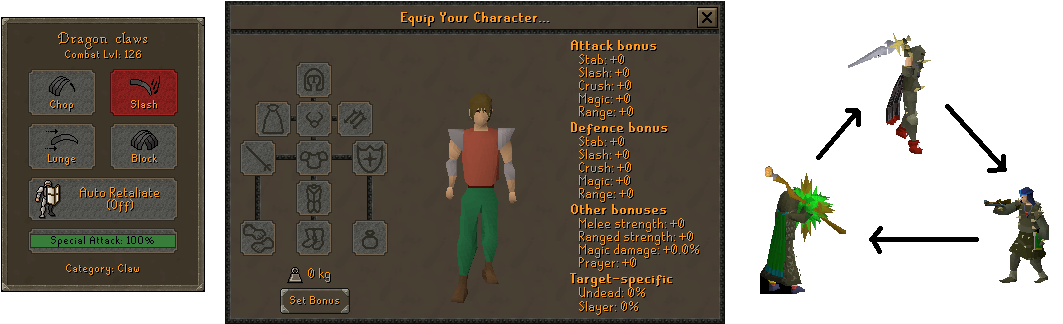
\includegraphics[width=\linewidth]{img/combat/Equipment_Stats_interface_and_triangle.png}
			\caption{The attack styles (left), equipment slots and associated equipment bonuses (middle) along with a depiction of the combat triangle (right). The attack styles for the \texttt{Dragon Claws} are Chop, Slash, Lunge, Block and give experience specifically to Attack, Strength, shared, and Defence, respectively. Shared means experience is split equally. In the equipment panel, the player is not wearing any equipment which results in 0 bonuses for all attributes. Starting with the bottom left of the combat triangle, a mage has advantage over the melee equipment typically worn by a melee fighter, a melee warrior has an advantage over the equipment typically worn by a ranged fighter, and ditto for ranged to mage.
			}
			\label{fig:equipment_stats_and_triangle}
		\end{figure}

	\subsection{Max Hits and Accuracy}
		Due to the large complexity and number of exceptions in the game, defining mathematical formulas for max hit and accuracy is very difficult/tedious. Instead, programming is the language for this. If you want to learn more about how max hits and accuracies are calculated see Ref.~\cite{bitter:dps_calculator}. You can also view a python translation of that code in the combat directory of the codebase accompanying this document.

	\subsection{Ticks and Attack Speed}
		At a fundamental level the entire game operates on a tick-based system. Every 0.6 seconds (called a tick) the game updates. This discretizes the possible game states, and typically means we will be dealing with sums in place of integrals, and recursive equations in place of differential equations.

		Once an attacker begins combat with an opponent, the fight continues until either is defeated, or one runs away. The attacks occur at an interval associated with the weapon. Different weapons have different \textit{Attack Speeds}, typically between 3-9 game ticks (1.8s - 5.4s). The attacker's attack speed $\mathcal{A}|s$, is the number of ticks between attacks. On each attack, the player's accuracy will determine the probability of a \textit{successful hit}. On a successful hit, a number between 0 and the player's maximum hit will be uniformly sampled as the damage the player does.

		A notable consequence of this tick-based system is that a series of precise player actions known as tick-manipulation allows players to perform multiple actions in a single tick, or to take advantage of mechanisms like tick-eating, allowing a player to survive otherwise fatal attacks.

	\subsection{Summary}
		A fighter has some combat skill levels and will (typically) equip some armour and a weapon. They will select an attack style, which selects the skill they will receive experience in, and which equipment bonuses plays a roll in the accuracy calculation. The problem then reduces to considering an accuracy and maximum hit. Once a fight begins, an attack occurs every couple of ticks. If the attack is successful, a uniform integer between 0 and their max hit is delivered to the opponent, reducing their current hit points. Once a fighter's health reaches 0, the fight is over.


\section{Agency}
	\subsection{Special Attacks}
		Certain weapons have the ability to use a special attack, typically dealing additional damage, but may also reduce the opponent's levels temporarily.

	\subsection{Temporary Boosts and Healing}
		Potions provide temporary boosts to skill levels.

	\subsection{Item Switching and Movement}
		Different items, moving around. Attack delays etc.
